\documentclass{article}
\usepackage{amsmath, amssymb, mdwlist, graphicx, hyperref}
\usepackage{listings,color}
\usepackage{wrapfig}
\usepackage[usenames,dvipsnames]{xcolor}
\definecolor{gray}{rgb}{0.97,0.97,0.97}
\lstset{%
language=C,%
%backgroundcolor=\color{gray},
emph={putpixel},
emphstyle=\bf,
tabsize=4,
framesep=5pt,
mathescape=true,
xleftmargin=0.1cm,
xrightmargin=0.1cm,
frame=lines,
%basicstyle=\ttfamily,
%keywordstyle=\color{Blue},
%commentstyle=\color{OliveGreen},
%stringstyle=\color{MidnightBlue},
columns=flexible,
%showstringspaces=false
}

\newcommand{\mpar}[1]{\marginpar{\textit{#1}}}
\newcommand{\norm}[1]{\Vert #1 \Vert}
\DeclareMathOperator{\argmax}{argmax}
\DeclareMathOperator{\argmin}{argmin}
\newenvironment{solution}{\paragraph{Solution.}$\,$ }{\vskip 3mm\hrule}
\newenvironment{exercise}[2]{\paragraph{Exercise #1 (#2pt).} }{
\medskip}
\newcommand{\bbR}{\mathbb{R}}
\newcommand{\bw}{\mathbf{w}}
\newcommand{\bx}{\mathbf{x}}
\newcommand{\bd}{\mathbf{d}}
\newcommand{\bb}{\mathbf{b}}
\newcommand{\by}{\mathbf{y}}
\newcommand{\bzero}{\mathbf{0}}
\newcommand{\bz}{\mathbf{z}}
\newcommand{\bSigma}{\mathbf{\Sigma}}
\newcommand{\bp}{\mathbf{p}}
\newcommand{\bP}{\mathbf{P}}
\newcommand{\bm}{\mathbf{m}}
\newcommand{\bc}{\mathbf{c}}
\newcommand{\bM}{\mathbf{M}}
\newcommand{\bV}{\mathbf{V}}
\newcommand{\bK}{\mathbf{K}}
\newcommand{\bD}{\mathbf{D}}
\newcommand{\bA}{\mathbf{A}}
\newcommand{\bX}{\mathbf{X}}
\newcommand{\bY}{\mathbf{Y}}
\newcommand{\bR}{\mathbf{R}}
\newcommand{\bI}{\mathbf{I}}
\newcommand{\bS}{\mathbf{S}}
\newcommand{\bT}{\mathbf{T}}
\newcommand{\balpha}{\boldsymbol{\alpha}}
\newcommand{\pt}[2]{\left(\begin{array}{c}#1\\#2\end{array}\right)}

\begin{document}
\title{MTAT.03.015 Computer Graphics (Fall 2013)\\
Exercise session XIV: OGRE}
\author{Konstantin Tretyakov, Ilya Kuzovkin}
\date{December 9, 2013}
\maketitle

In this exercise session we will have a look at high-level graphics engine called OGRE\footnote{\url{http://www.ogre3d.org/}}. We will see how the concepts we know about are included into the OGRE engine making our life easier: lighting, materials, shadows, environmental mapping and other techniques are made accessible by adding few lines of code, without the need to implement all annoying details on our own.

The solutions will have to be submitted as a zipped project directory. Please do not remove Windows libraries if you work on Linux and vice versa.

\section{Structure of the application}
We start by comparing the structure of the application to the familiar structure we've been using so far. Please open \verb#1_OgreTriangle# project and read through the code in the \verb#triangle.cpp# file. Compare it to the GLUT-based applications we have seen before.

\begin{exercise}{1}{0.5}
Add a small square which will fly around the triangle and rotate around it's own center. For that you will need to
\begin{enumerate}
	\item Create a new \verb#Ogre::ManualObject# object using \verb#createManualObject()# method of the scene manager.
	\item Describe vertices of you square. Look up in the documentation of the \\
\verb#Ogre::RenderOperation# class\footnote{\url{http://www.ogre3d.org/docs/api/html/classOgre_1_1RenderOperation.html}} which operation type you should use. Note that in OGRE we first create the vertex itself and then describe it's attributes.
	\item Create \verb#Ogre::SceneNode# and attach the new object to it.
	\item Use this \verb#SceneNode# to animate our object (update it's potision) in the \verb#frameRenderingQueued()# method, which is an analog of \verb#idleFunc()# in GLUT.
\end{enumerate}
The existing code for the triangle will serve you as example. The result should look something like this:
\begin{center}
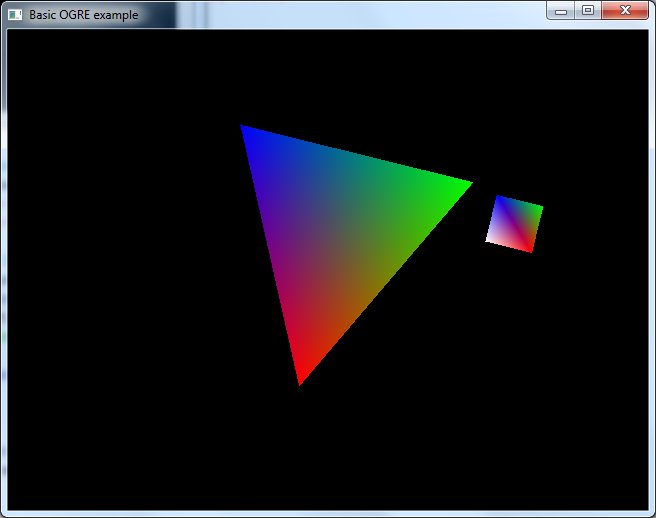
\includegraphics[width=0.7\textwidth]{ex1.png}
\end{center}
\end{exercise}

%\begin{exercise}{2}{0.5}
%You may have noticed that all objects on the scene are associated with \verb#Ogre::SceneManager# object. The whole scene, including objects, their locations (through \verb#Ogre::SceneNode#), cameras, lights and so on, is described and stored using screen manager. This provides us with a natural way to define several scenes.
%In this exercise you need to add second scene to the application, put any object of your liking in there and use spacebar to toggle between the scenes.
%\end{exercise}

\section{High-levelness}

Open project \verb#2_OgreLight#

\begin{exercise}{2}{0.5}
Add light and material. Lots of instructions here or leave partial code.
\end{exercise}

\begin{exercise}{3*}{0.5}
Add a plane and a stencil shadow
\end{exercise}

\ \\
Open project \verb#3_OgreMesh#

\begin{exercise}{4}{0.5}
Shadow mapping. Is it hard?
\end{exercise}

\begin{exercise}{5}{1}
Skybox with sky texture. Or any other texture (are there many of them in OGRE?)
\end{exercise}

\begin{exercise}{6*}{1}
Make mesh reflective. So that it will reflect this skybox
\end{exercise}


\section{Plugins}

Open project \verb#4_OgrePlugins#. You can switch scenes, look how it's done.

\begin{exercise}{6}{0.5}
Do ??? with particle system
\end{exercise}

\begin{exercise}{6*}{1}
Add some other plugin (or any other display of creativity?)
\end{exercise}


\end{document}
